\documentclass[crop, tikz]{standalone}
\usepackage{tikz}

\usetikzlibrary{calc,decorations.pathmorphing,positioning}

\begin{document}
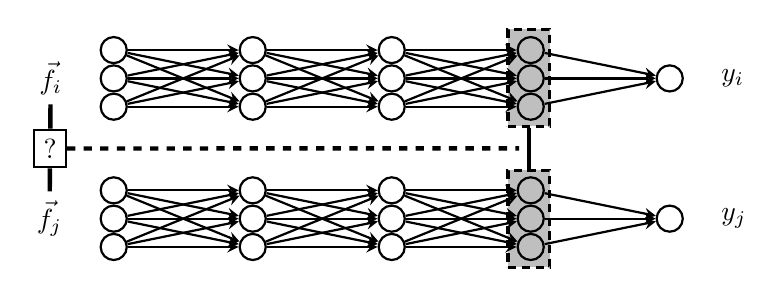
\begin{tikzpicture}
	\node[very thick, densely dashed, draw=black,rectangle, minimum height=3.5em, minimum width=1.5em, xshift=15em, yshift=-1em, fill=lightgray] (rekt1) {};
				
	\node[very thick, densely dashed, draw=black,rectangle, minimum height=3.5em, minimum width=1.5em, xshift=15em, yshift=-6.1em, fill=lightgray] (rekt2) {};
				
	\draw[ultra thick] (rekt1) -- (rekt2);
				
	\node[] (c) at ($(rekt1)!0.5!(rekt2)$) {};
				
	\node[circle, draw, thick] (f11) {};
	\node[circle, draw, thick, below=0em of f11] (f12) {};
	\node[circle, draw, thick, below=0em of f12] (f13) {};
	\node[circle, draw, thick, below=2em of f13] (f21) {};
	\node[circle, draw, thick, below=0em of f21] (f22) {};
	\node[circle, draw, thick, below=0em of f22] (f23) {};
				
	\node[left=1em of f12] (il1) {$\vec{f}_i$};
	\node[left=1em of f22] (il2) {$\vec{f}_j$};
				
	\node[rectangle, draw, thick] (Q) at ($(il1)!0.5!(il2)$) {?};
	\draw[ultra thick] (il1) -- (Q);
	\draw[ultra thick] (il2) -- (Q);
				
	\draw[dashed, ultra thick] (Q) -- (c);
				
	\node[circle, draw, thick, right=4em of f11] (h11) {};
	\node[circle, draw, thick, right=4em of f12] (h12) {};
	\node[circle, draw, thick, right=4em of f13] (h13) {};
	\node[circle, draw, thick, right=4em of f21] (h21) {};
	\node[circle, draw, thick, right=4em of f22] (h22) {};
	\node[circle, draw, thick, right=4em of f23] (h23) {};
				
	\node[circle, draw, thick, right=4em of h11] (k11) {};
	\node[circle, draw, thick, right=4em of h12] (k12) {};
	\node[circle, draw, thick, right=4em of h13] (k13) {};
	\node[circle, draw, thick, right=4em of h21] (k21) {};
	\node[circle, draw, thick, right=4em of h22] (k22) {};
	\node[circle, draw, thick, right=4em of h23] (k23) {};
				
	\node[circle, draw, thick, right=4em of k11] (l11) {};
	\node[circle, draw, thick, right=4em of k12] (l12) {};
	\node[circle, draw, thick, right=4em of k13] (l13) {};
	\node[circle, draw, thick, right=4em of k21] (l21) {};
	\node[circle, draw, thick, right=4em of k22] (l22) {};
	\node[circle, draw, thick, right=4em of k23] (l23) {};
				
	\node[circle, draw, thick, right=4em of l12] (o1) {};
	\node[circle, draw, thick, right=4em of l22] (o2) {};
	\node[right=1em of o1] (ll1) {$y_i$};
	\node[right=1em of o2] (ll2) {$y_j$};
				
	\foreach \l in {1,2}
		\foreach \x in {1,2,3}
			\foreach \y in {1,2,3}
				\draw[-stealth, thick] (f\l\x) -- (h\l\y);
				
	\foreach \l in {1,2}
		\foreach \x in {1,2,3}
			\foreach \y in {1,2,3}
				\draw[-stealth, thick] (h\l\x) -- (k\l\y);
				
	\foreach \l in {1,2}
		\foreach \x in {1,2,3}
			\foreach \y in {1,2,3}
				\draw[-stealth, thick] (k\l\x) -- (l\l\y);
				
	\foreach \l in {1,2}
		\foreach \x in {1,2,3}
			\draw[-stealth, thick] (l\l\x) -- (o\l);

\end{tikzpicture}
\end{document}